\chapter*{Opis teoretyczny algorytmu ewolucyjnego}
Proces uczenia sygnalizacji świetlnej w tej pracy został zrealizowany z pomocą algorytmu ewolucyjnego. Ten rozdział opisuje kolejne kroki, z których składa się proces uczenia. Szczegóły dotyczące implementacji poniższego algorytmu zostały opisane w następnym rozdziale.
\section*{Pierwsze pokolenie}
Przebieg uczenia rozpoczyna się od wygenerowania pierwszego pokolenia osobników. Osobnik to właściwie zbiór wartości określonych parametrów. W pierwszym pokoleniu wartości te generowane są losowo, z zakresu określonego w konfiguracji algorytmu. 
\section*{Funkcja dostosowania}
Osobniki wygenerowanego pokolenia poddawane są ocenie, która określa ich dostosowanie (ang. \textit{fitness}). Funkcja dostosowania określona jest wzorem:
\[ f(x) = max(t(1),\ldots, t(n)) - t(x)\]
gdzie:\\
\begin{tabularx}{\textwidth}{ r c l }
$x$ & -- & oceniany osobnik\\
$n$ & -- & liczba osobników w pokoleniu\\
$t(a)$ & -- & czas, w jakim określona liczba samochodów przejechała przez skrzyżowanie,\\ &&przy sygnalizacji ustawionej wg parametrów osobnika $ a $
\end{tabularx}
\section*{Generowanie nowego pokolenia}
Wybór osobników do nowego pokolenia odbywa się drogą selekcji turniejowej. Z poprzedniego pokolenia losowane są 3 osobniki. Spośród tych trzech wybierany jest ten o najwyższej wartości funkcji dostosowania. Taki turniej powtarzany jest $2n$ razy, gdzie $n$ to liczba osobników w pokoleniu (określona w konfiguracji algorytmu). Następnie ze zbioru $2n$ osobników wybieranych jest $n$ o najlepszej wartości funkcji dostosowania. Ta pula poddana jest następnie krzyżowaniu lub mutacji.
\section*{Krzyżowanie i mutacja}
Każdy osobnik z wygenerowanej puli zostaje zmutowany albo skrzyżowany z innym osobnikiem. Decyduje o tym ważone losowanie. Prawdopodobieństwo, że osobnik zostanie poddany mutacji jest zmienne i wyznacza je funkcja:
\[ f(x) = (sin(x * \frac{1}{\frac{g}{1000}+\frac{x}{100}})+1) : 2 \]
gdzie:\\
\begin{tabularx}{\textwidth}{ r c l }
	$x$ & -- & numer obecnego pokolenia\\
	$g$ & -- & liczba wszystkich pokoleń, określona w konfiguracji algorytmu\\
	&&\\
\end{tabularx}\\
Wykres tej funkcji przedstawiono na rysunku~\ref{fig:mutRate}. \\ Po zastosowaniu krzyżowania lub mutacji nowe pokolenie jest gotowe do oceny funkcją dostosowania opisaną wcześniej.

\begin{figure}[h]	
	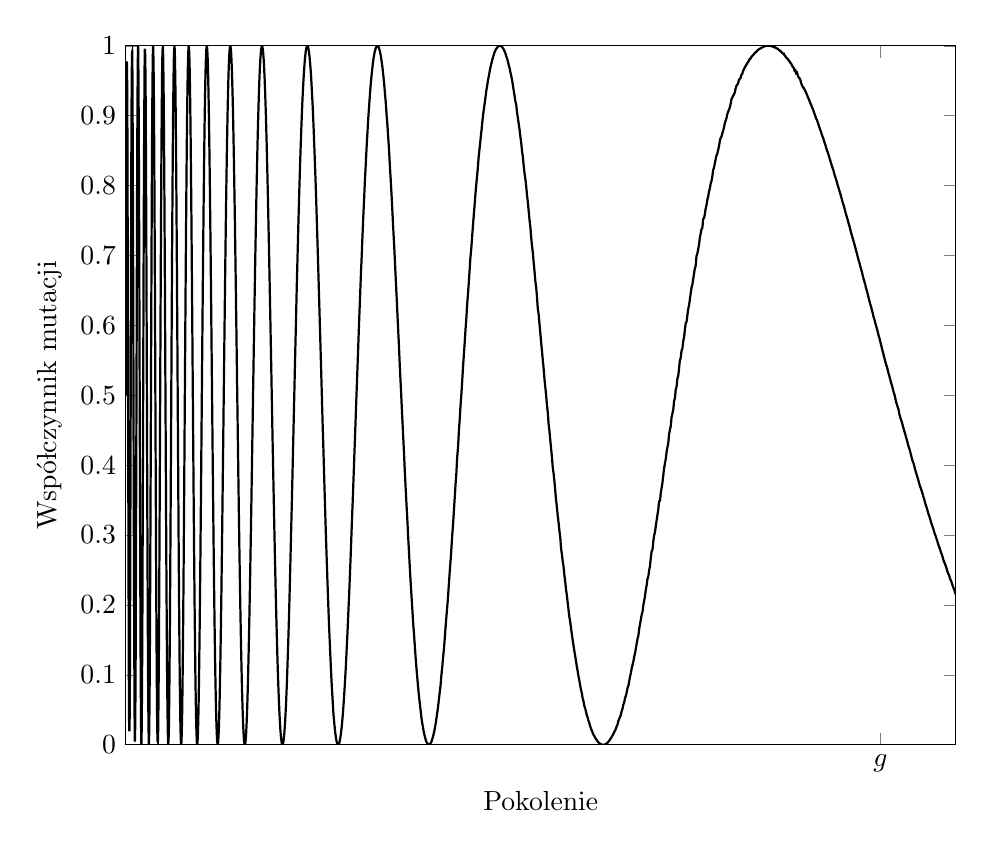
\begin{tikzpicture}
	\begin{axis}
	[
	domain=0:110,
	width=\textwidth,
	xlabel=Pokolenie,
	ylabel=Współczynnik mutacji,
	xmin=0,
	xmax=110,
	ymin=0,
	ymax=1,
	samples=1000,
	xtick=100,
	xticklabel={$g$},
	smooth
	]
	\addplot+[mark=none,thick, black]{(sin(x * (1 / (0.1 + (x / 100.0)))*(180/3.14)) + 1.0)/2.0};
	\end{axis}
	\end{tikzpicture}
	\caption{Funkcja określająca współczynnik mutacji}
	\label{fig:mutRate}
\end{figure}